%%%%%%%%%%%%%%%%%%%%%%%%%%%%%%%%%%%%%%%%%%%%%%%%%%%%%%%%%%%%%%%%%%%%%%%%%%%%%%%%
%%%%%%%%%%%%%%%%%%%%%%%%%%%%%%%%%%%%%%%%%%%%%%%%%%%%%%%%%%%%%%%%%%%%%%%%%%%%%%%%
%%%%%%%%%%%%%%%%%%%%%%%%%%%%%%%%%%%%%%%%%%%%%%%%%%%%%%%%%%%%%%%%%%%%%%%%%%%%%%%%
\chapter{Herramientas y técnicas de análisis}
\label{cha:tools}
%%%%%%%%%%%%%%%%%%%%%%%%%%%%%%%%%%%%%%%%%%%%%%%%%%%%%%%%%%%%%%%%%%%%%%%%%%%%%%%%
%%%%%%%%%%%%%%%%%%%%%%%%%%%%%%%%%%%%%%%%%%%%%%%%%%%%%%%%%%%%%%%%%%%%%%%%%%%%%%%%
%%%%%%%%%%%%%%%%%%%%%%%%%%%%%%%%%%%%%%%%%%%%%%%%%%%%%%%%%%%%%%%%%%%%%%%%%%%%%%%%

\section{Herramientas de simulación}

La importancia de tener una muestra de datos simulados tiene diversos motivos. Primeramente, permite entrenar a las herramientas que después se usarán sobre datos reales, pero teniendo conocimiento completo del proceso estudiado. Por otra parte, el proceso de detección es preciso, pero no perfecto, lo que produce que aparezcan desviaciones en las distribuciones físicas. Para tener en cuenta estos efectos, y corregirlos, se emplean simulaciones completas de \lhcb del canal en concreto a estudiar: el \emph{full} Monte Carlo.

En \lhcb la aplicación \color{dieg} encargada \color{norm} de llevar a cabo la generación y transporte de partículas a través del detector es \textsc{Gauss} \cite{Clemencic_2011}. Esta herramienta funciona en dos bloques separadamente que pueden ser operados en conjunto (\emph{vid.} Figura \ref{fig_gaussapp}):
\begin{itemize}
	\item Generación de eventos: Las colisiones protón--protón son generadas usando \pythia \cite{sjostrand2015introduction}, con una configuración específica para \lhcb. Las desintegraciones de partículas son descritas con \eviltgen \cite{Lange:2001uf} y la radiación de las partículas en el estado final son generadas por \photos \cite{golonka2006photos}.
	\item Simulación del detector: La interacción entre las partículas generadas con el detector, y la respuesta de este mismo, la describe \geant \cite{Agostinelli:2002hh}.
\end{itemize}


El proceso de generación y reconstrucción de trazas es computacionalmente costoso y se realiza en el GRID de \lhcb. 
El GRID de \lhcb se compone de una red internacional de computadores conectados cuyo objetivo principal es el análisis de datos del experimento. Al sistema de computación distribuida puede accederse desde \textsc{Dirac} o mediante \textsc{Ganga}, dos herramientas que hacen de interfaz con el usuario y el sistema de colas.

%Este es un hecho de capital importancia puesto que, de este modo, estos recursos son comunes a todos los físicos que analizan datos.


%De hecho, la cantidad limitada de MC viene siendo la principal contribución a la incertidumbre sistemática de $\phi_s$.


\begin{figure}[H]
\centering
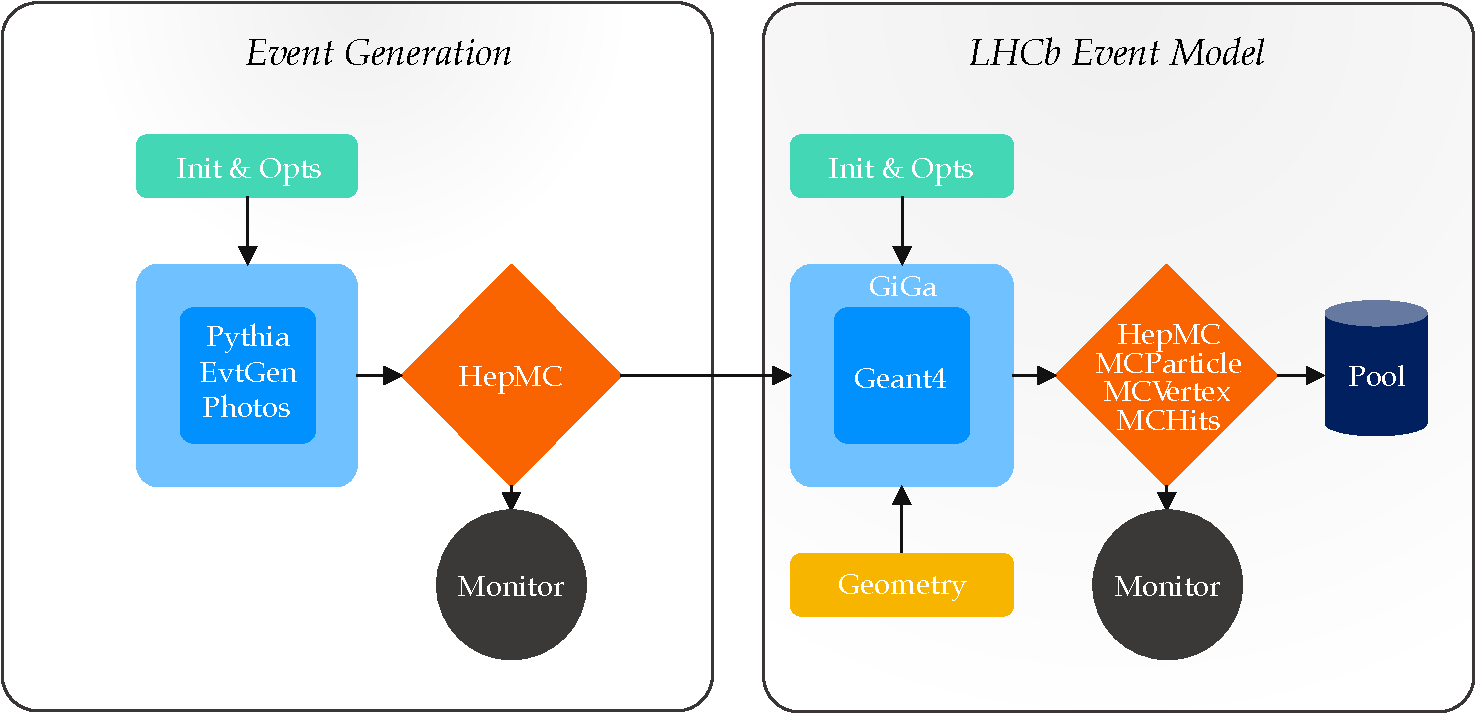
\includegraphics[width=0.95\textwidth]{GaussApplication.pdf}
\caption{Estructura de la aplicación  \textsc{Gauss}.}	 \label{fig_gaussapp}
\end{figure}




\subsection{Modelo para $\Bs \rightarrow \Jpsi \kaon \antikaon$} %%%%%%%%
\label{sec:Bs2JpsiKKmodel}

En el marco concreto de este trabajo se creó un nuevo modelo de \texttt{EvtGen}, para simular el canal $\Bs \rightarrow \Jpsi \kaon \antikaon$, con capacidad para crear y desintegrar las resonacias $\fzero$, $\fai$ y $\ftwop$, y \color{vero} generar también la interferencia entre ellas. \color{norm} 

El modelo debe incorporar las distribuciones angulares de la \S \ref{sec_angdist}, la evolución temporal de la \S \ref{sec_tempdist}, y las distribuciones de masa para las partículas de ondas S (no resonante), S ($\fzero$), P($\fai$) y D($\ftwop$), que aparecen en \S \ref{sec_diffrate}.  Todas estas funciones se escriben en \texttt{C++}, y se adecúan para ser integradas en el software de \lhcb, \textsc{Gauss}. Para poder interaccionar con el modelo, se compone también un \texttt{DecFile}, en el cual se escribe la lista de parámetros que constituyen la entrada al simulador.

\begin{table}[H]
\centering
\resizebox{\textwidth}{!}{\begin{tabular}{r|c|c|c|c|c|l}
nombre del canal & $f$ &$f_f$ & $\delta$ & $\phi_s$ &$\lambda$  \\ \hline
\texttt{1.0    mu+ mu-  K+    K-     BS\_MUMUKK} 
%
&   \texttt{0.00},& & \texttt{0.00,}& \texttt{-0.8,}& \texttt{1.0,}	\\
&  \texttt{0.50,} &                 & \texttt{3.32,}& \texttt{-0.8,}& \texttt{1.0,} \\
  &  \texttt{0.50,} & \texttt{0.509,} & \texttt{0.00,}   &\texttt{-0.8,} &  \texttt{1.0,}\\ 
  &                 & \texttt{0.260,} & \texttt{3.08,} & \texttt{-0.8,} & \texttt{1.0,} \\
 &                 &                 & \texttt{3.26,} & \texttt{-0.8,} & \texttt{1.0,}\\
 &                 & \texttt{0.468,} & \texttt{0.00,}   & \texttt{-0.8,} & \texttt{1.0,}\\
 &                 & \texttt{0.194,} & \texttt{3.08,} & \texttt{-0.8,} & \texttt{1.0,}\\
 &                 &                 & \texttt{3.26,} & \texttt{-0.8,}& \texttt{1.0,} &
 \texttt{0.6603, 0.08, 17.7,        
0.9499, 0.99, 1.05;}\\ \hline
&&&&&& $\Gamma$ \hspace*{6.5mm} $\Delta \Gamma$  \hspace*{4mm} $\Delta m$  \hspace*{2mm} $$   \hspace*{3mm}$m_{f_0} $\,\,\,$m_{\text{KK}}^{\text{mín}}$   $m_{\text{KK}}^{\text{máx}}.$  %\hspace*{0.2mm}
\end{tabular}}
\caption{Parámetros y valores de los mismos declarados en el \texttt{DecFile}. Se puede hallar una descripción detallada en el texto.} \label{tab:decfiles}
\end{table}

El primer bloque que se indica en ta Tabla \ref{tab:decfiles} indica el nombre del canal y las partículas involucradas. El siguiente bloque controla los parámetros de la distribución angular, las fracciones, fases y parámetros de violación CP. La primera columna, $f$, son las fracciones de cada una de las amplitudes onda S, P y D; por normalización se construye la fracción de onda D como $f_{D} = 1-f_{S}-f_{P}$. La segunda columna, $f_f$ indica la fracción de cada polarización que existe en una amplitud dada, por ejemplo la fracción de $f_{P\parallel} = 1-f_{P0}-f_{P\perp} = 1-0.509-0.260$. Seguidamente en la tercera y cuarta columna se definen $\delta$ y $\phis$, una para cada polarización y en radianes. La quinta columna de este bloque indica el parámetro de violación CP, $|\lambda|$, definiéndose uno para cada polarización. El último bloque controla la parte de la mezcla y desintegración, $\Gamma\,(\mathrm{ps^{-1}})$ , $\Delta \Gamma \,(\mathrm{ps^{-1}})$ y $\Delta m \,(MeV/)c^2$); el valor del polo de $\fzero$, $m_{f_0}$ (GeV/$c^2$); así como la ventana de masa en la que se generan los datos, $[m_{\text{KK}}^{\text{mín}},m_{\text{KK}}^{\text{máx}}]$ (GeV/$c^2$).


\begin{figure}[H]
\begin{flushright}
\begin{multicols}{2}
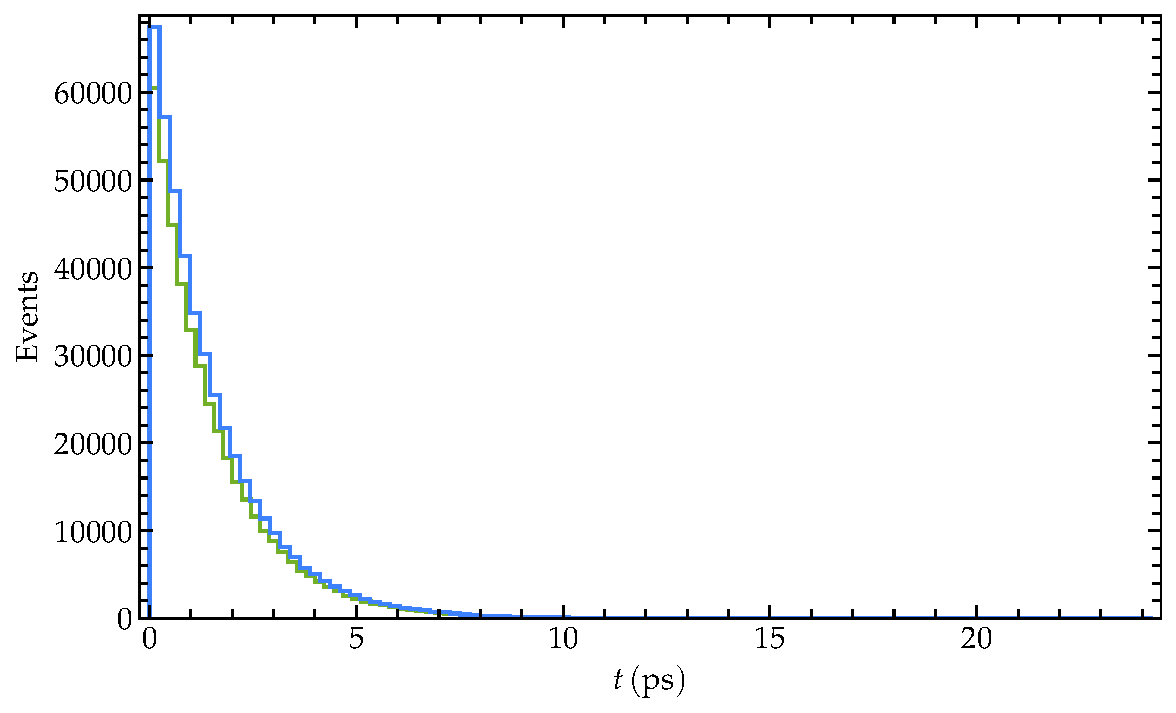
\includegraphics[width=\columnwidth]{plots/time} \\
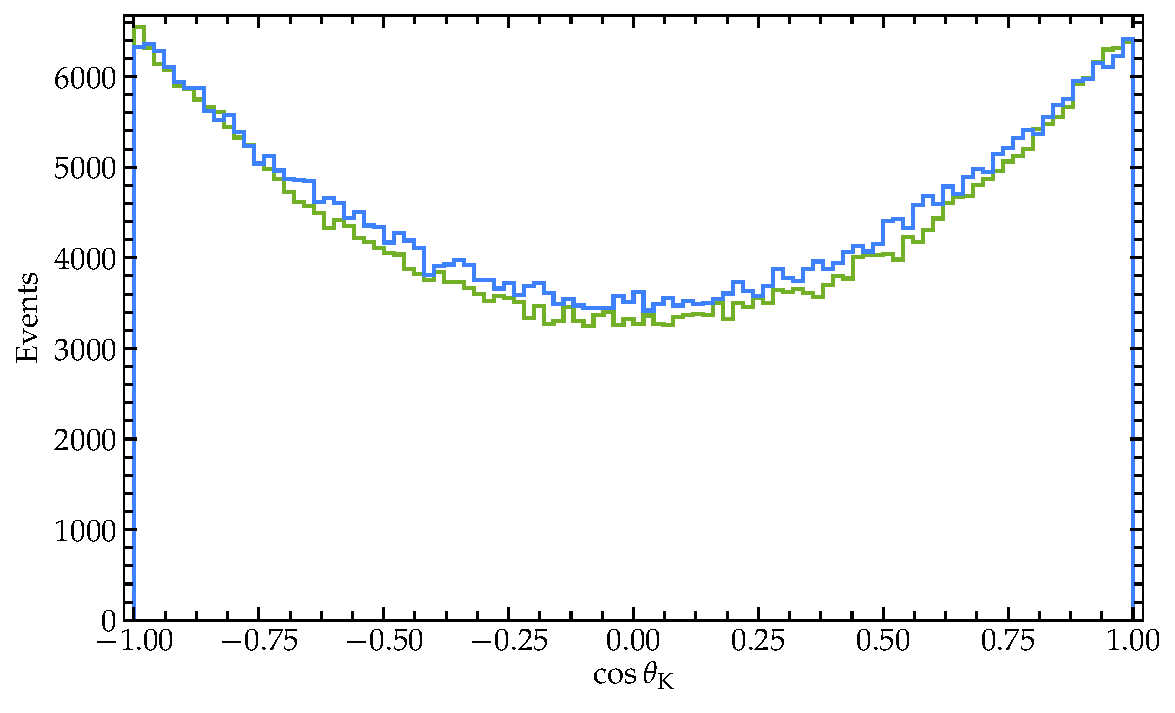
\includegraphics[width=\columnwidth]{plots/hel_costhetaK} \\
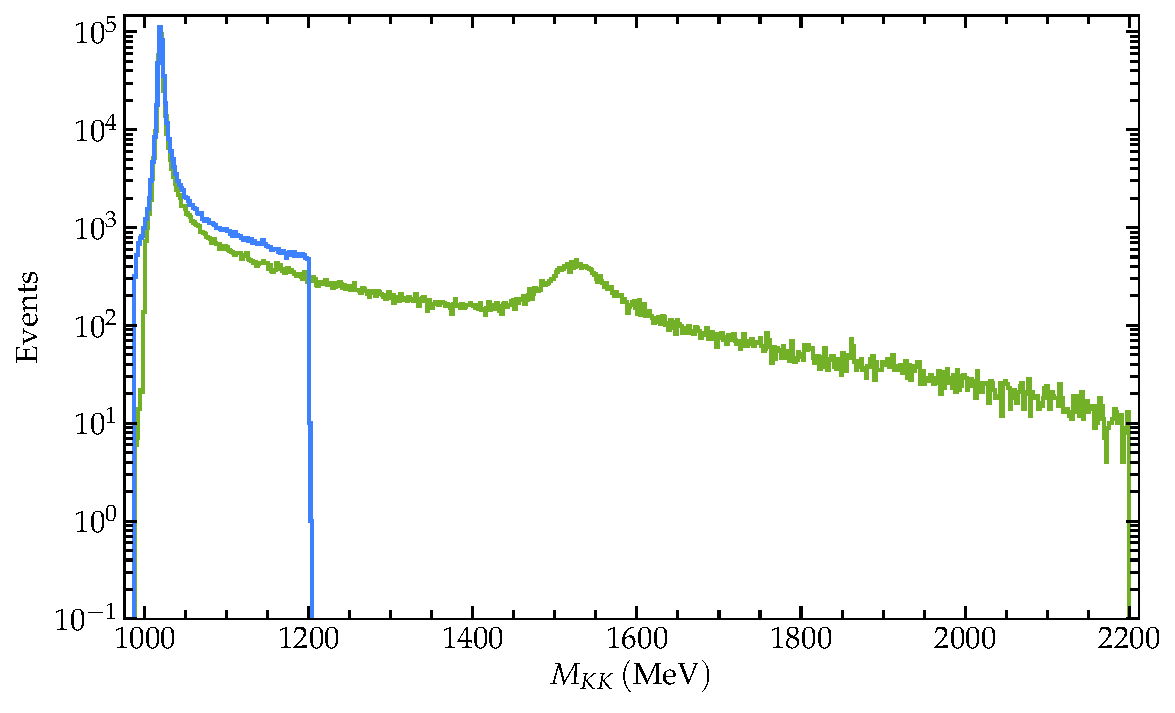
\includegraphics[width=\columnwidth]{plots/mkk} \\
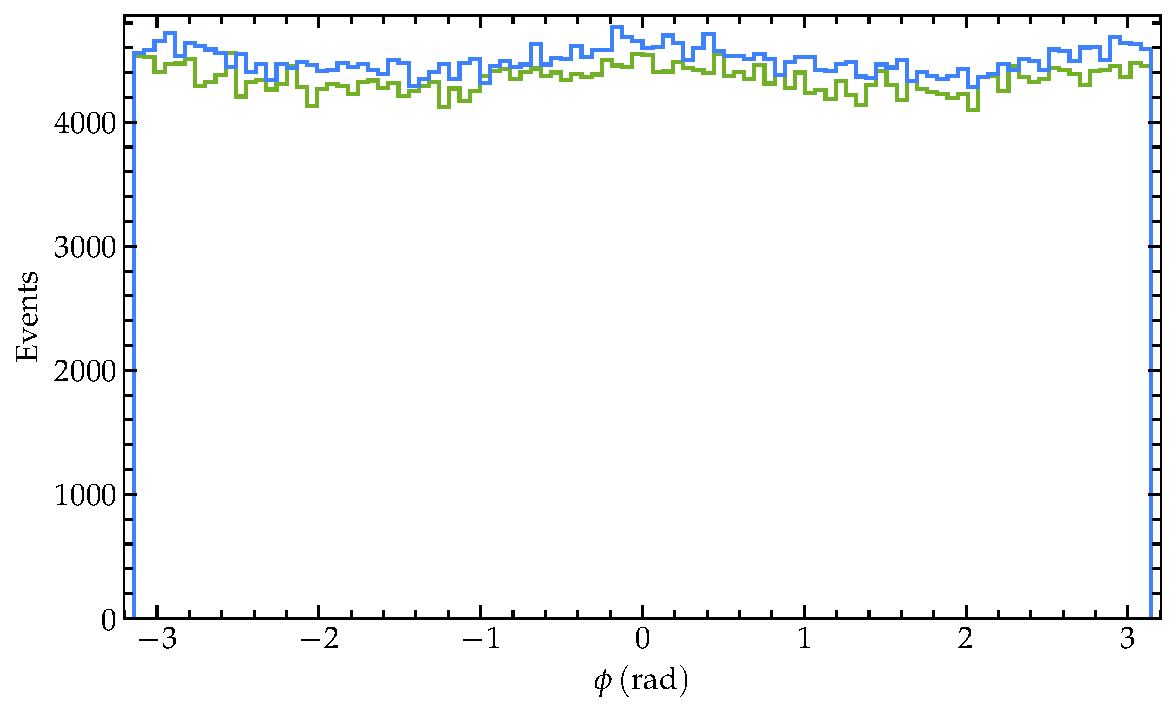
\includegraphics[width=\columnwidth]{plots/hel_phi} \\
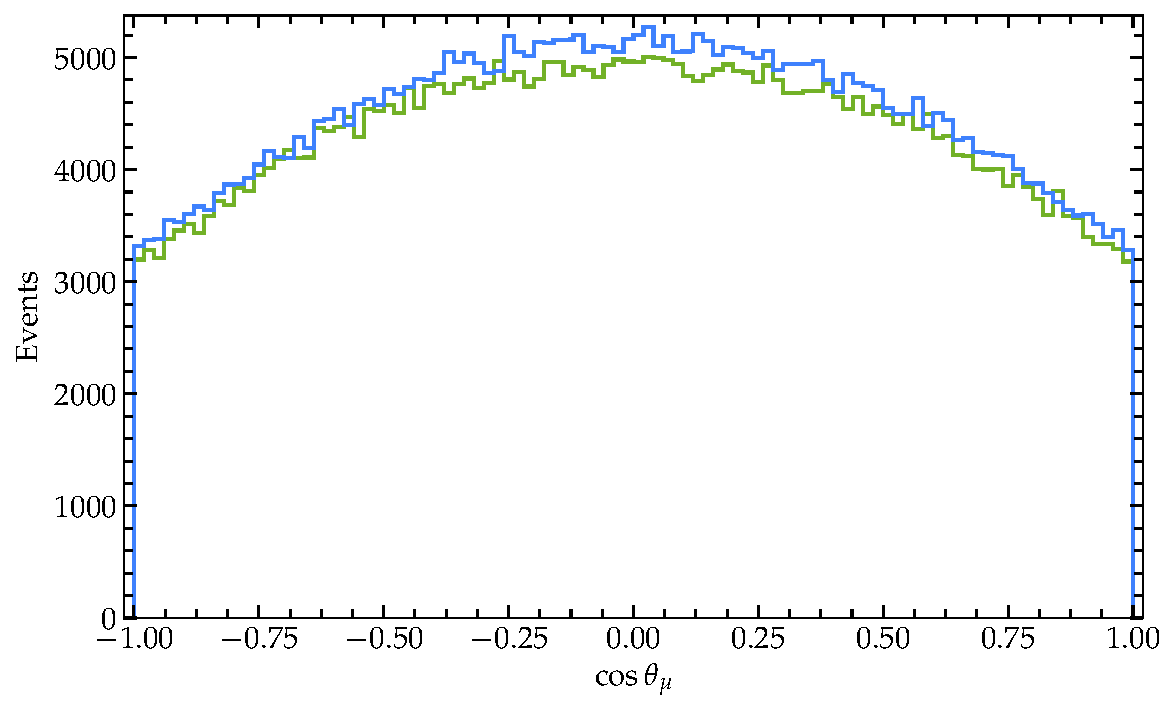
\includegraphics[width=\columnwidth]{plots/hel_costhetamu} \\
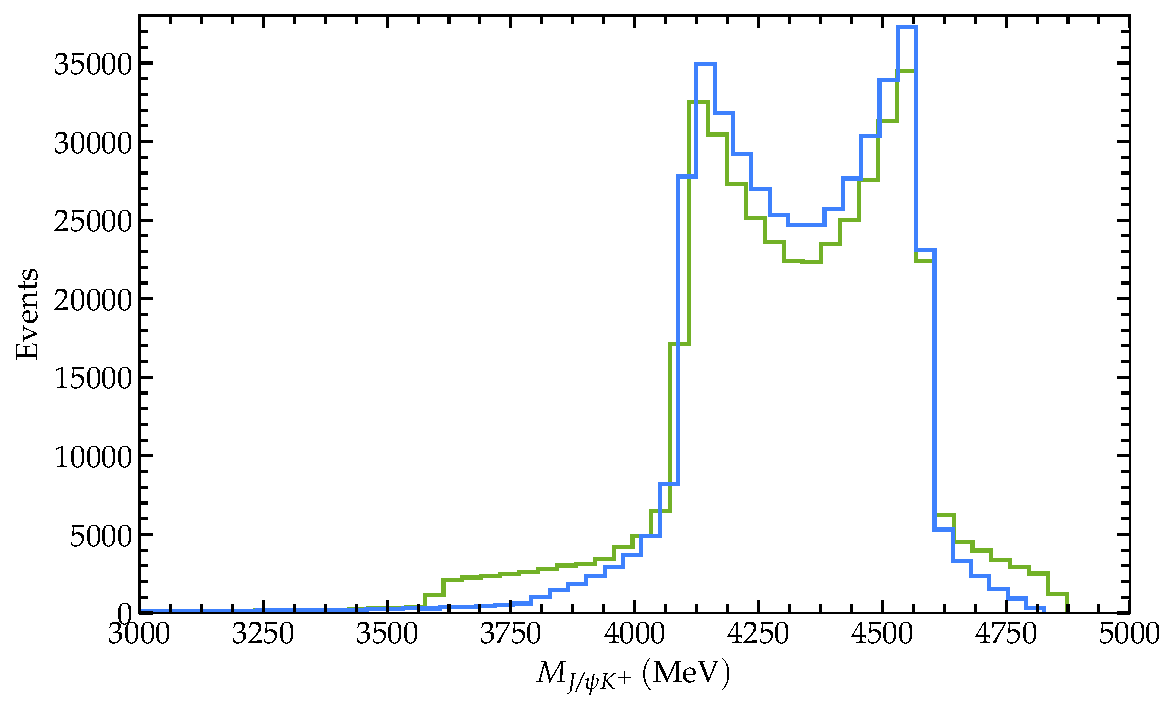
\includegraphics[width=\columnwidth]{plots/mjpsik}
\end{multicols}
\end{flushright}
\caption{Histogramas de algunas de las variables simuladas. Las muestras de $5\times10^5$ eventos  son \emph{sin} onda D (azul), con $7\,\%$ S onda y $93\,\%$ P \emph{wave} en la ventana de masa $m_{\text{KK}} = [0.98,1.20]\,\mathrm{GeV}/c^2$; y \emph{con} onda D (verde), con $15\,\%$ S \emph{wave} y $70\,\%$ P \emph{wave} y $15\,\%$ D \emph{wave} en el rango de masa $m_{\text{KK}} = [1.0,2.2]\,\mathrm{GeV}/c^2$.}   \label{fig_evtgensamples1}
\end{figure}


En la \S \ref{sec_diffrate}, se calcula la tasa de decaimiento diferencial respecto de los ángulos de helicidad y del tiempo, y pueden verse muestras generadas con \textsc{Gauss} en la Figura \ref{fig_evtgensamples1}. \textsc{Gauss} genera los cuadrimomentos de las partículas, llamados vectores Lorentz, 
\[p_{\mu} = (p_0, \vec{p}) = (Ec^{-1},\vec{p})\]
de modo que es sencillo calcular la masa, empleando la \emph{pseudo}norma del vector de Lorentz
\[p^{\mu}p_{\mu} = \frac{E^2}{c^2} - |\vec{p}|^2 = m^2c^2. \]
Entonces, para el espectro de masa $\kaon\antikaon$, se suman las componentes los momentos de los dos kaones calculándose la masa con el cuadrivector suma; análogamente para el $\Jpsi\kaon$, se suman las del $\kaon$ y de los muones.

En la Figura \ref{fig_evtgensamples2} puede observarse el espacio fásico en el Dalitz \textit{plot} que representa $M_{\Jpsi\kaon}$ \emph{vs.} $M_{\kaon \antikaon}$, y donde se aprecian las diferentes contribuciones que fueron implementadas.





\begin{figure}[H]
\centering
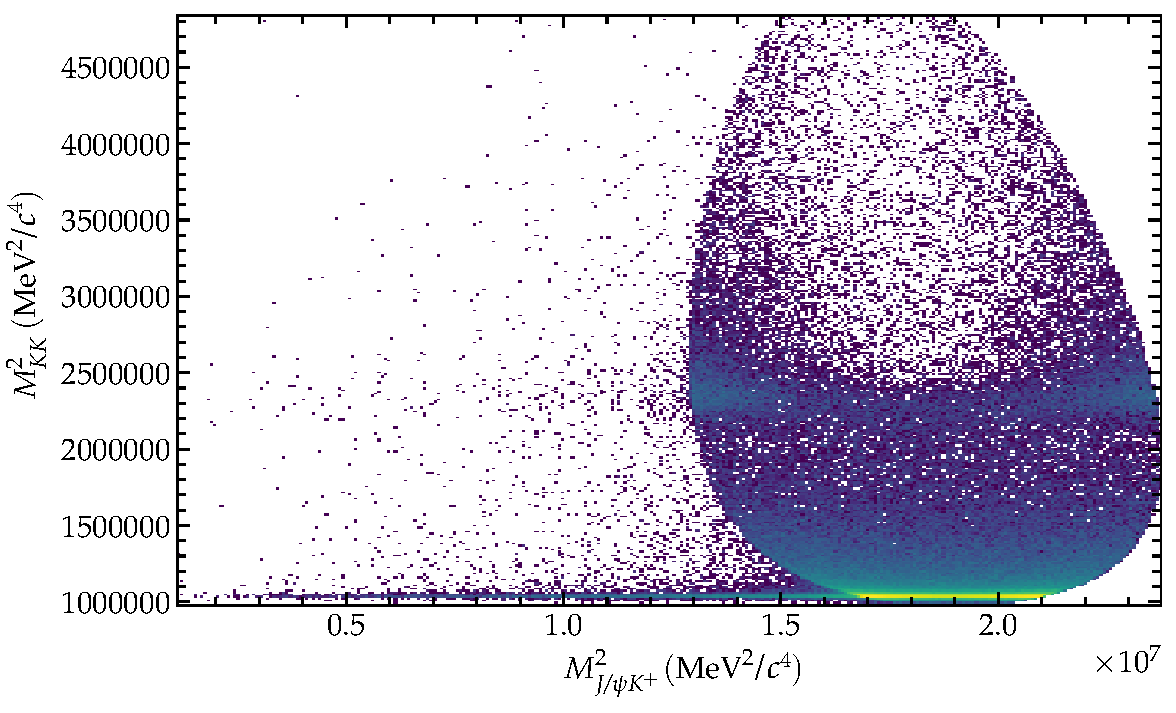
\includegraphics[width=0.9\textwidth]{plots/dalitz1}
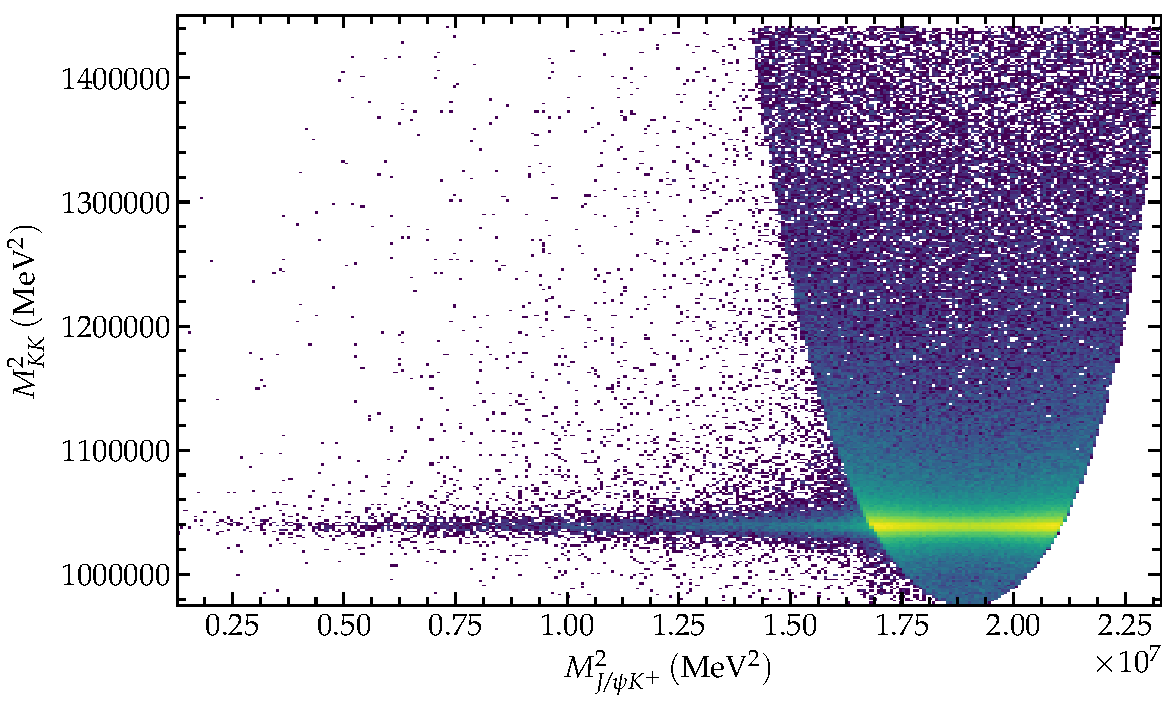
\includegraphics[width=0.9\textwidth]{plots/dalitz2}
\caption{Dalitz \textit{plot} para dos muestra de $5\times 10^5$ eventos, arriba con $15\,\%$ S \emph{wave}, $70\,\%$ P \emph{wave} y $15\,\%$ D \emph{wave} y abajo $11\,\%$ S \emph{wave}, $89\,\%$ P \emph{wave}. Se aprecian claramente las resonancias $\fai$ y $\ftwop$. Alrededor del $\fai$, puede verse también $\fzero$ de una forma más difusa.}   \label{fig_evtgensamples2}
\end{figure}




%%TODO wave -> onda

\color{norm}



\section{Estimación por máxima verosimilitud}

\color{new}
Para extraer parámetros de conjuntos de datos, como las que se muestran en la Figura \ref{fig_evtgensamples1}, se emplean algoritmos de ajuste (\emph{fit}). Existen diversos métodos para poder minimizar un funcional respecto de una muestra y extraer los parámetros, entre ellos aquí se emplea el método de máxima verosimilitud.

\color{norm}

El método de máxima verosimilitud \cite{cowan}, MLE, es una técnica para estimar los valores de parámetros \emph{verdaderos}, $\theta_k^0$, de una muestra finita de datos, $x_i$, dada. Si la medida se repite $N$ veces, entonces $x_i$ tendrá $N$ valores para la dimensión $i$ (pudiendo tener una variable más dimensiones).



Asumiendo la hipótesis de la función de densidad de probabilidad, \emph{p.d.f.}, para la muestra $x$, y siendo todas las medidas independientes, se verifica que
\begin{equation}
\text{probabilidad de } \quad x_i \in [x_i, x_i+dx_i] \quad \forall i \quad  = \quad \prod_{i=1}^N f(x_i,\theta_k) dx_i	
\end{equation}




Si la hipótesis es correcta y los parámetros son $\theta_k \approx \theta_k^0$, se espera una alta probabilidad para los datos medidos. Mismamente, si los parámetros se alejan del valor verdadero $\theta_k^0$, entonces se obtendrá una baja probabilidad.
Como  $dx_i$ no depende de los parámetros, se define la función de verosimilitud como
\begin{equation}
	L(\theta_k) = \prod_{i=1}^N f(x_i,\theta_k) \label{eq_likelihood_def}
\end{equation}  
que no es más que la \color{dieg} $p.d.f.$ conjunta de $x_i$ como función de los parámetros a estimar. \color{norm} Los datos actúan como constantes, puesto que el experimento ha finalizado.


En virtud de la Ecuación (\ref{eq_likelihood_def}), 
uno define el método de máxima verosimilitud (MLE), escogiendo maximizar la función de verosimilitud, \emph{likelihood}. Se trata por tanto de buscar
\begin{equation}
	\frac{\partial L(\theta_k)}{\partial \theta_k} = 0, \qquad k=\{1,\dots,N\}.
\end{equation}

\begin{figure}[H]
\centering
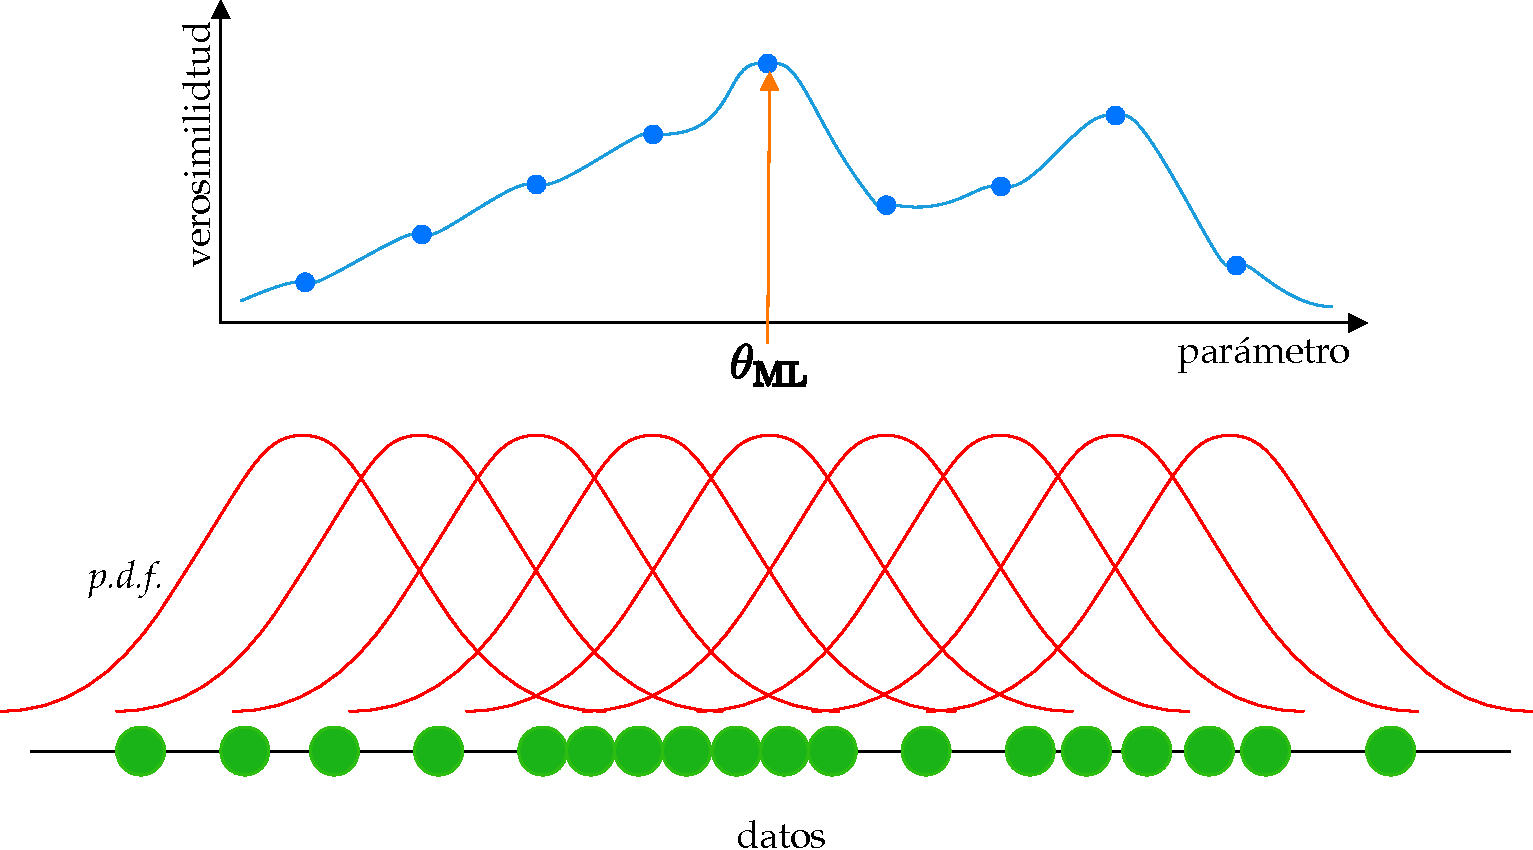
\includegraphics[width=0.9\textwidth]{MLfit.pdf}
\caption{Ejemplo conceptual del ajuste por máxima verosimilitud. Se ajustan unos ciertos datos respecto de una \textit{p.d.f.} gaussiana, cuyo valor del parámetro media coincide con la media de la muestra, y ello se corresponde con el máximo de la veroslimilitud.} \label{fig_maxloglikeexp}
\end{figure}	
%TODO make new picture here






\section{Minimizar}

Para realizar los ajustes por máxima verosimilitud, se requiere de un algoritmo capaz de encontrar extremos relativos de funciones que sea lo suficientemente sofisticado para manejar grandes cantidades de datos y funciones de varios parámetros. 


\subsection{Paralelización}



\color{dieg}
Gran parte del coste computacional  del análisis recae en el cálculo de la \emph{likelihood}, que luego se optimiza.  
%
La minimización puede ser un proceso lento, sobre todo con grandes cantidades de datos y parámetros, y más cuando se procede vía un ajuste multidimensional. Es aquí donde la paralelización se vuelve de gran ayuda. Típicamente una CPU tiene del orden de 10 \textit{cores}, en los que se pueden paralelizar procesos, mientras que una GPU tiene del orden de 100 veces más \textit{cores}. 

La paralelización se realiza por eventos, calculándose la \emph{likelihood} en la GPU para cada conjunto de parámetros y llevándose a cabo la minimización en la CPU con \minuit \cite{James:1975dr},  un minimizador de tipo gradiente que busca mínimos de funciones y es reconocido como uno de los mejores algoritmos de su tipo. 
\color{norm}

Para este trabajo se emplearon GPUs de la marca \textsc{nVidia}, y que son relativamente fáciles de usar, puesto que la propia compañía ofrece \textsc{cuda}, un \textit{framework} que permite usar las tarjetas programando en \texttt{cuda}--\texttt{C}, muy similar a \texttt{C}.
%
Al final se emplea \texttt{Python} como una interfaz y gestor de datos en la CPU, empleando para ello la librería \texttt{PyCuda}; existiendo además un paquete de software llamado \texttt{Ipanema} \cite{santos2017ipanema}, con funcionalidades adecuadas a esta línea de trabajo. Desde el punto de vista técnico, se necesita de la CPU para coordinar todos los procesos y de un código que la GPU entienda, en donde se indiquen las posiciones y operaciones que deben hacerse sobre \emph{arrays} de datos, así como una forma óptima de salida del programa. Puede verse un esquema de como operan las diferentes parte en la Figura \ref{fig:CPUioGPU}.





\begin{figure}[H]
  \centering
  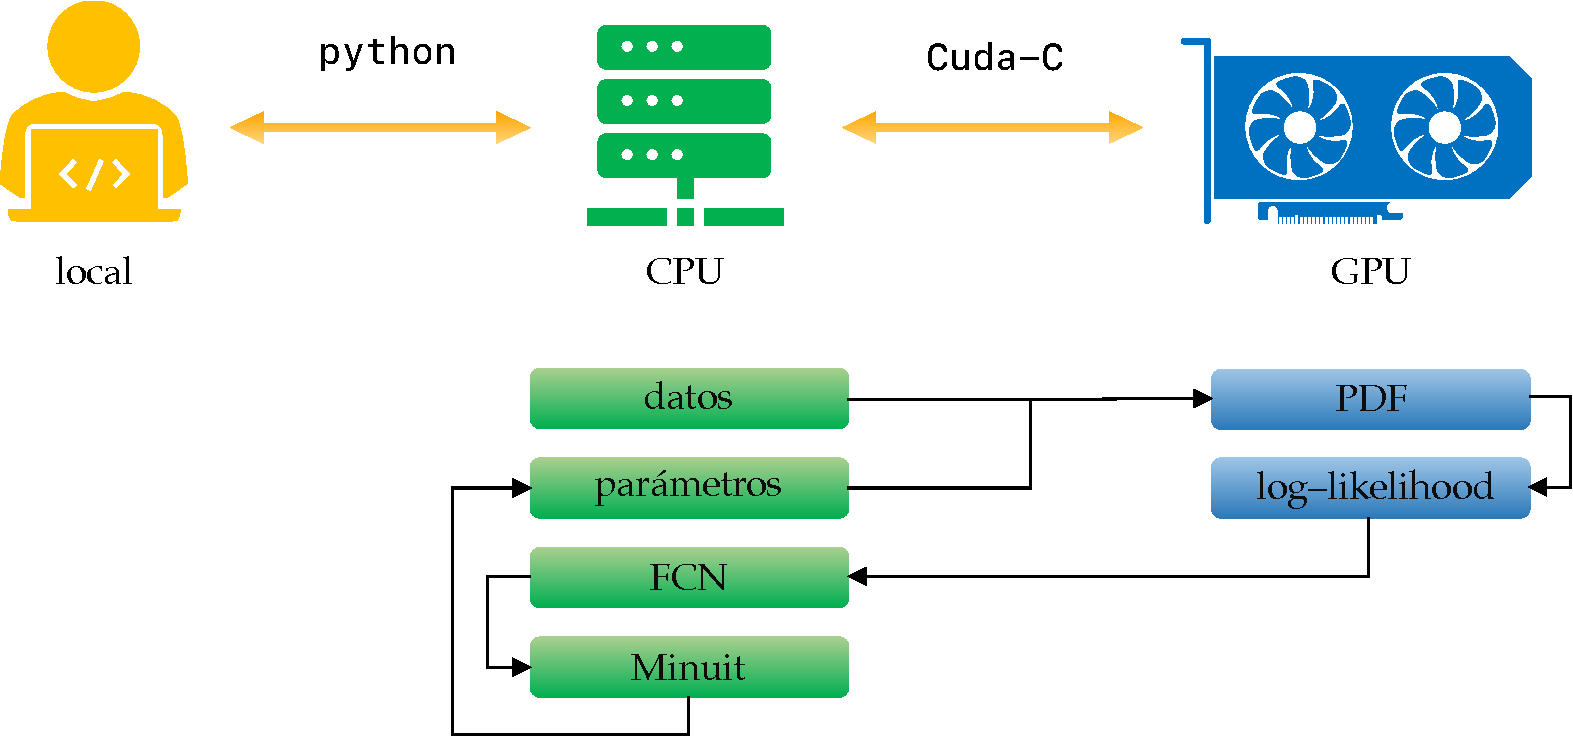
\includegraphics[width=0.9\textwidth]{CPUioGPU.pdf}
  \caption{Esquema del flujo de trabajo e interacciones entre el usuario, la CPU y la GPU con \texttt{Ipanema}. Aquí FCN se refiere al valor de la función a cada llamada de la CPU, y es el número a minimizar con Miniuit.} \label{fig:CPUioGPU}
\end{figure}


\subsection{Minuit}

\texttt{Minuit} es un algoritmo escrito por F. James en la década de los 70 en el CERN. Fue concebido como una herramienta para encontrar el mínimo de funciones multiparamétricas y analizar la forma de la función alrededor del mínimo. Su principal aplicación es el análisis estadístico de datos, principalmente para obtener el mejor conjunto de parámetros que minimice un $\chi^2$ o maximice la verosimilitud. Además de estimar los parámetros, computa sus incertidumbres estadísticas y la correlación entre ellos. Es especialmente útil para problemas difíciles, incluyendo aquellos que requieran de ser guiados para hallar la solución correcta 
\cite{James:1975dr}.

Brevemente, las funciones que \texttt{Minuit} aporta son:
\begin{itemize}
  \item \texttt{Migrad}: Encuentra, empleando la fórmula Davidon–Fletcher–Powell (DFP), el conjunto de parámetros que minimiza un funcional dado sobre unos datos.
  \item \texttt{Hesse}: Estima con mayor precisión la hessiana, extrayéndose de esta parte las incertidumbres parabólicas de los parámetros obtenidos con \texttt{Migrad}.   
  \item \texttt{Minos}: En problemas complicados es plausible que la función a minimizar no sea simétrica respecto de un parámetro alrededor del mínimo (como presupone \texttt{Hesse}), por ello esta función, computacionalmente más costosa, estima la incertidumbre asimétrica de los parámetros.
\end{itemize}



\subsection{Fórmula de Davidon–Fletcher–Powell}

El algoritmo DFP fue desarrollado por Davidon (1959), Fletcher y Powell (1963), y es también conocido como el \emph{variable metric algorithm} \cite{fletcher1963rapidly}. Se trata de una generalización de los métodos \textit{quasi}--Newton, que asegura que se preserve que la hessiana sea definida positiva.

Considérense la función $f(x)$ y su gradiente $\nabla f$, y la matriz hessiana $H$, la serie de Taylor de la función $f$ es \cite{fletcher2000practical}
\begin{equation}
  f(x_k+s_k) = f(x_k) + \nabla f(x_k)^T s_k + \frac{1}{2} s_k^{\top} {H} s_k + \dots,
\end{equation}
y para su gradiente (ecuación secante), que es usado para calcular la hessiana es
\[\nabla f(x_k+s_k) = \nabla f(x_k) + H s_k + \dots\,.\]
  

La fórmula DFP encuentra la solución a la ecuación secante que es más próxima al valor estimado y que además verifica la condición de curvatura, cumpliendo que la hessiana sea simétrica y definida positiva
\begin{equation}
  H_{k+1}=
(I - \gamma_k y_k s_k^{\top}) H_k (I - \gamma_k s_k y_k^{\top}) + \gamma_k y_k y_k^{\top},
\end{equation}
donde $y_k = \nabla f(x_k+s_k) - \nabla f(x_k),$ con 
$\gamma_k = \frac{1}{y_k^{\top} s_k}$.

A cada iteración la aproximación a la inversa de la hessiana $G_k = G_k^{-1}$ es
\begin{equation}
  G_{k+1} = G_k - \frac{G_k y_k y_k^{\top} G_k}{y_k^{\top} G_k y_k} + \frac{s_k s_k^{\top}}{y_k^{\top} s_k}.
\end{equation}
donde se asume que $H$ es definida positiva, cumpliendo los vectores  $s_k^T$ e $y$ la condición de curvatura
\begin{equation}
  s_k^{\top} y_k = s_k^{\top} H s_k > 0.
\end{equation}

La fórmula DFP es muy efectiva, y de hecho fue el primer método \textit{quasi}--Newton en generalizar el método de la secante para un problema multidimensional. Sin embargo, para grandes problemas no cuadráticos, el algoritmo puede estancarse; un fenómeno atribuido a que $H$ se vuelve una matriz casi singular. Notar que a pesar de ello es mejor la fórmula Broyden--Fletcher--Goldfarb--Shanno, que es dual (bajo el intercambio $y$ y $s$).



\begin{figure}[H]
  \centering
  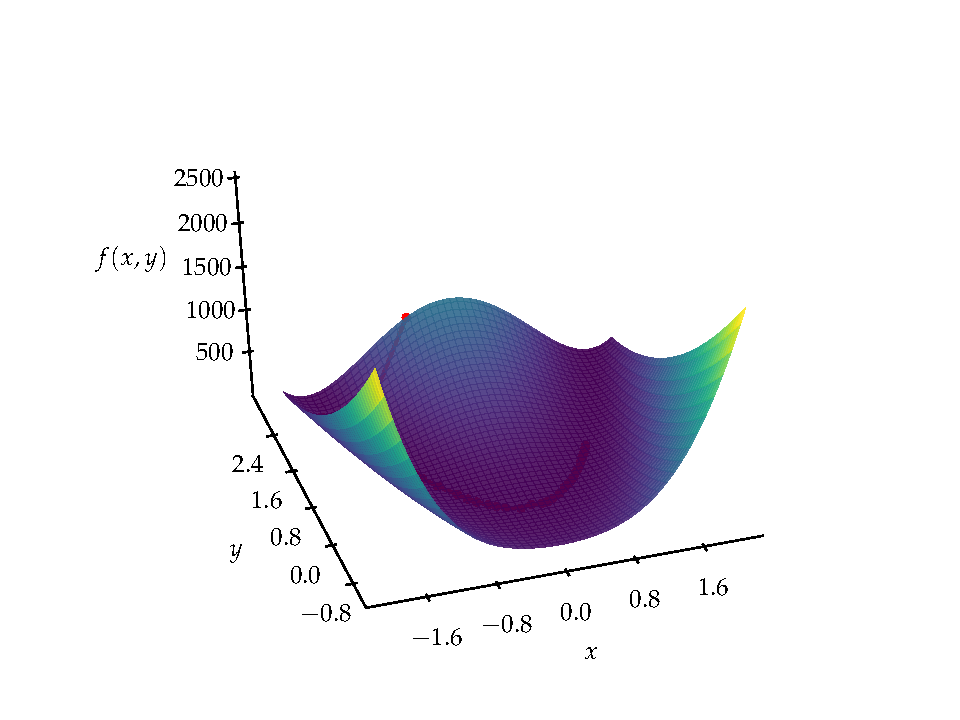
\includegraphics[width=0.7\textwidth]{rosen.pdf}
  \caption{Minimización de la función de Rosenbrock mediante el método DFP. Se situó la semilla en $(-0.5,3)$, y se halló el mínimo de $f(x, y) = (a-x)^2 + b(y-x^2)^2$ en $(1,1)$ para los parámetros $a=1$ y $b=100$.}
\end{figure}



\section{Splines}

Los splines son funciones polinómicas definidas a trozos, que resultan particularmente útiles para interpolar datos con formas complicadas y que pueden tener ruido. Existen diferentes formas de construir splines, aquí se centrará el texto en los \textit{basis} splines con polinomios de tercer orden.


\subsection{B-splines}

Dado un conjunto de nodos, $k = \{u_0,\dots,u_n\}$, con $n+1$ elementos que definen $n$ intervalos, para un spline cúbico hay $n+3$ parámetros, $b$, que lo definen \cite{Weisstein}. La función interpolante  se construye como la suma lineal de b--splines \cite{paperPhis}
\begin{equation}
s(u) = \sum_{i=0}^{n+2}  b_i s_i(u).
\end{equation}
%
Para un valor $u$ en un determinado intervalo, $u \in (u_i,u_{i+1}]$, contribuyen cuatro b--splines, concretamente, $s_i(u)$ con $i \in \{i,i+1,i+2,i+3\}$. Es preciso extender los nodos en los extremos para calcular dichas contribuciones,
\[u_{i} = u_0 \,\,\, \forall i<0 \qquad \text{y} \qquad u_{i} = u_{n} \,\,\, \forall i>n.\]

Definiendo, la variable $\delta$ \cite{paperPhis},
\begin{equation}
  \delta_i(u) = u - u_i \qquad \qquad \delta_i^j = u_j -u_i
\end{equation}
se pueden escribir las cuatro contribuciones no nulas como,
\begin{equation}
  s_i(u) = b_i A_i(u) + b_{i+1} B_i + b_{i+2} C_i + b_{i+3} D_i 
\end{equation}
donde
\begin{equation}
\begin{split}
  A_i(u)&= -\frac{ \delta_{i+1}(u) ^3}
                 { \delta_{i-2}^{i+1} \delta_{i-1}^{i+1} \delta_{i  }^{i+1}}\\
  B_i(u)&=  \frac{ \delta_{i-2}(u) \delta_{i+1}(u)^2 }
                 { \delta_{i-2}^{i+1} \delta_{i-1}^{i+1} \delta_{i  }^{i+1}} 
           +\frac{ \delta_{i-1}(u) \delta_{i+1}(u) \delta_{i+2}(u) }
                 { \delta_{i-1}^{i+2} \delta_{i-1}^{i+1} \delta_{i  }^{i+1}} 
           +\frac{ \delta_{i}(u) \delta_{i+2}(u)^2 }
                 { \delta_{i  }^{i+2} \delta_{i-1}^{i+2} \delta_{i  }^{i+1}} \\
  C_i(u)&=  \frac{ \delta_{i-1}(u)^2 \delta_{i+1}(u) }
                 { \delta_{i-1}^{i+2} \delta_{i-1}^{i+1} \delta_{i  }^{i+1}} 
           +\frac{ \delta_{i-1}(u) \delta_{i}(u) \delta_{i+2}(u) }
                 { \delta_{i  }^{i+2} \delta_{i-1}^{i+2} \delta_{i  }^{i+1}} 
           +\frac{ \delta_{i}(u)^2 \delta_{i+3}(u) }
                 { \delta_{i  }^{i+3} \delta_{i  }^{i+2} \delta_{i  }^{i+1}} \\
  D_i(u)&=  \frac{ \delta_{i}(u) ^3}
                 { \delta_{i  }^{i+3} \delta_{i  }^{i+2} \delta_{i  }^{i+1}}.
\end{split}
\end{equation}
De este modo, fijando un conjunto de nodos, se han de encontrar los parámetros $b$. Por simplicidad a la hora de ser implementado, es útil considerar
\begin{equation}
   b_i A_i(u) + b_{i+1} B_i + b_{i+2} C_i + b_{i+3} D_i = \beta_0 + \beta_1 u + \beta_2 u^2 + \beta_3 u^3
\end{equation}
donde los coeficientes $\beta_i$ son propios de cada bin, a diferencia de los $b_i$, que son comunes a todo el spline. 


%\begin{equation}
%  P = \delta_{i-2}^{i+1} \delta_{i-1}^{i+1} \delta_{i  }^{i+1}
%  Q = \delta_{i-1}^{i+2} \delta_{i-1}^{i+1} \delta_{i  }^{i+1}
%  R = \delta_{i  }^{i+2} \delta_{i-1}^{i+2} \delta_{i  }^{i+1}
%  S = \delta_{i  }^{i+3} \delta_{i  }^{i+2} \delta_{i  }^{i+1}
%\end{equation}

%\subsection{\emph{Smoothing} splines}
%
%Los \textit{smoothing} splines son funciones de estimación que se obtienen a partir de una cierta muestra de observaciones $y_i$  para un determinado modelo $f(x_i)$ \cite{reinsch1967smoothing}.
%
%Considerando un conjunto de nodos (\emph{knots}) $\{k_i\}_{i=0}^{n-1}$ y que existe la relación $y_i = f(k_i) + \epsilon_i$ , donde $\epsilon_i$  son variables aleatorias de media cero y de varianza constante. El \textit{smoothing} spline $\hat{f}$ es la estimación de la función $f$, penalizando el salto de la segunda derivada
%\begin{equation}
%\chi^2(\lambda) = \sum_{i=0}^{n-1} \left(\frac{y_i - \hat f(x_i)}{\sigma_i}\right)^2 + \lambda \int \hat f''(x)^2 \,dx,
%\end{equation}
%donde $\lambda$ es el parámetro de suavizado que controla la relevancia de la integral de las segundas derivadas.
%
%A medida que $\lambda \rightarrow 0$, el \textit{smoothing} spline converge al spline interpolante. Por otra parte, según $\lambda \rightarrow \infty$, la penalización sobre las rugosidades se vuelve cada vez más importante y el \textit{smoothing} spline converge a un ajuste  lineal por mínimos cuadrados.
%
%Con los splines se puede suavizar el ruido en datos $(x_i,y_i)$, resultando en splines menos rugosos. Resulta particularmente interesante el caso de los splines cúbicos, que además de su buen funcionamiento, simplifican el proceso \cite{paperPhis}. 
%
%
%
%\subsubsection*{B--splines cúbicos suavizados}
%
%Si se consideran b-splines cúbicos, entonces el término de penalización se simplifica. Como los coeficientes de los splines están totalmente determinados por los $\hat f (k_i)$, el problema se puede separar en dos partes:
%\begin{enumerate}%[(i)]
%  \item Obtener un conjunto de puntos $(k_i,\mu_i = \hat f (k_i))$, construyendo un spline interpolante entre $(k_i,y_i)$.
%  \item A partir de $\mu_i$, construir un B--spline $ \hat{f}(x)$, para todo $x$.
%\end{enumerate}
%
%Como la derivada segunda de un B--spline cúbico es una función lineal, entonces se sigue que el término de penalización se puede escribir como una forma cuadrática,
%\begin{equation}
%\int \hat f''(x)^2 dx = \mu^{\top} \textbf{M} \,\mu.
%\end{equation}
%donde la matriz $\textbf{M}$ (de dimensión $n\times n $), puede expresarse como $\textbf{M} = \textbf{V}^{\top} \textbf{W}^{-1} \textbf{V}$. 
%%
%%
%La matriz $\textbf{V}$, de dimensión $(n-2)\times n$, y se construye con elementos de segundas diferencias,
%\begin{equation*}
%V = \begin{pmatrix}
%\frac{1}{h_1} & -\left(\frac{1}{h_1}+\frac{1}{h_{2}}\right) & \frac{1}{h_{2}} & 0 & \cdots & 0 \\
%0 & \frac{1}{h_i} & -\left(\frac{1}{h_i}+\frac{1}{h_{i+1}}\right) & \frac{1}{h_{i+1}} & \cdots & 0 \\
%\vdots & \vdots & \ddots & \ddots & \ddots & \vdots \\
%0 & 0 & \cdots & \frac{1}{h_{n-2}} & -\left(\frac{1}{h_{n-2}}+\frac{1}{h_{n-1}}\right) & \frac{1}{h_{n-1}} 
%\end{pmatrix}
%\end{equation*}
%%
%%
%La matriz $\textbf{W}$, simétrica, tridiagonal y de dimensión $(n-2)\times(n-2)$, se construye con las distancias entre nodos sucesivos
%\begin{equation*}
%W = \begin{pmatrix}
%\frac{h_0+h_{1}}{3}  & \frac{h_0}{6} & 0 & \cdots & 0 \\
%\frac{h_i}{6} & \frac{h_i+h_{i+1}}{3}  & \frac{h_i}{6} & \cdots & 0 \\
%\vdots & \ddots & \ddots & \ddots & \vdots \\
%0 & 0 & \cdots & \frac{h_{n-3}}{6} & \frac{h_{n-3}+h_{n-2}}{3} 
%\end{pmatrix}
%\end{equation*}
%
%
%Entonces se aplica el paso (\textsc{i}) y la suma de cuadrados se puede escribir como
%\[\chi^2(\lambda) = \sum_{i=0}^{n-1} \left(\frac{y_i - \hat f(x_i)}{\sigma_i}\right)^2 + \lambda \vec{\mu}^{\top} \textbf{M} \,\vec{\mu}. \]
%Esto implica que $\chi^2 (\lambda)$ es una función de segundo orden en $\mu$ y por lo tanto su minimización resulta de optimizar el sistema 
%\begin{equation}
%  \left(\Sigma^{-1} - \lambda \textbf{M} \, \right) \mu = \Sigma^{-1} Y, \qquad \Sigma^{-1} = \text{diag}(1/\sigma_i).
%\end{equation}
%Resolviendo dicho sistema, se puede obtener un conjunto \textit{smooth} $\mu_i$, que luego se puede usar para construir un B--spline interpolante ---paso (\textsc{ii}).
%
%








